\chapter{Methodology}

\label{chapter:methodology}

% Camera calibration
% This is done by knowing the 3D position of each interest point and it's projections (colored sircles on \autoref{fig:calib}), and after taking a sample of images on a static camera and the pattern moving along X and Y axis with different scale and skew.
% Then some algorithm can be used to estimate unknown parameters of a calibration matrix, for example: estimate the camera projection matrix (can be done from 6 correspondences) and decompose it to $R$, $\vec{t}$ and $K$ 

% The problem solution can be divided into several steps. 
% Firstly, it is necessary to make a math model of a device that can solve the problem and describe its behaviour. 
% The next step is to make a CAD model of the cameras' holder, print and assemble it, and then calibrate it. 
% Then detect features and compute the distance to visible objects in cameras' overlapping zone: as far as a stereo pair is calibrated, the precision depends on a stereo pair calibration, cameras' calibration, key point extractor and matcher.
% As a result, provided points and features can be used in an SfM algorithm to correct a relative stereo pair position in time while moving and in a feedback loop inside the MRS system to correct its path planning concerning found obstacles.
\begin{figure}[h]
    \centering
    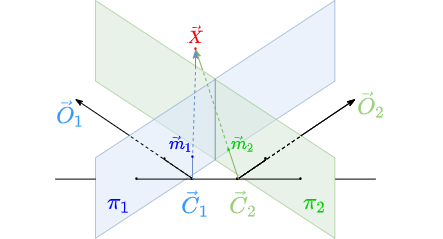
\includegraphics[width=.7\textwidth]{graphics/td90deg.png}
    \caption{Scheme of stereovision}
    \label{fig:td90deg}
\end{figure}

\section{General multicamera calibration}

\section{Features extraction and matching}

\section{Features pose estimation}

